\section{Tangible User Interfaces in Visualization}
The purpose of this chapter is to introduce Tangible User Interfaces which are settled in the domain of visualization. We will give an overview of TUIs in visualization we consider noteworthy. In the previous chapter, some of the presented TUIs could also be labeled as TUIs for visualization, because some output is visualized by the system. In the reacTable for example, the sound waves between different musical objects are visualized on the table-top. However, the reacTable is designed as a musical instrument. In this chapter, we will focus explicitly on TUIs, which sole purpose is the visualization of data.

\subsection{Tangible Views for Information Visualization}
Tangible Views is a TUI for information visualization presented by \cite{spindler10}. It consists of several handheld displays, which allow to interact with the visualized data in a more direct way. Similar to Paper Windows, a TUI presented by \cite{holman05}, the information is project onto cardboard displays (Tangible Views) as well as a table-top. The setup also consists of several IR cameras, which track the Tangible Views and make them spatially aware. Gestures performed on the Tangible View are recognized by the system as well. Tangible Views are enhanced with IR markers, to simplify tracking. The cardboard displays are cheap in production. Figure \ref{fig:tangible_views} shows applications of Tangible Views in practice.

\begin{figure*}[htb]
\centering
\includegraphics[width=0.95\textwidth]{figures/tangible_views.png}
\caption{Tangible Views in practice (compare \protect\cite{spindler10})}
\label{fig:tangible_views}
\end{figure*}

The stationary table-top display, which can be of arbitrary size and shape, acts as a contextual background. Graphical information is displayed on the table-top display. In this information space, the Tangible Views serve as local views in the context of the table-top display. Tangible Views can be used with other Tangible Views simultaneously. They can be seen as a multiple view environment with each Tangible View representing a unique physical view into a virtual information world. This makes them an ideal tool for collaboration or comparison tasks. Since Tangible Views can be easily produced, different shapes may contribute to different visualization tasks and take a special role during interaction.

\subsubsection{Interacting with Tangible Views}
The design of Tangible Views was aimed at an easy and natural usage, which is inspired by everyday life interaction principles. The interaction takes place within the physical space defined by the table-top display. In this three-dimensional space, Tangible Views are moved around by the users and provide appropriate feedback. Six degrees of freedom are available for interaction, this includes the position and the local rotation of the Tangible View. Corresponding interactions are translation and rotation, which are easy to learn and simple to execute.

\cite{spindler10} define eight interaction techniques for interaction with Tangible Views. The interaction techniques have been tailored to fit the needs of information visualization. Some of the techniques rely heavily on the available six degrees of freedom. The following eight techniques are defined in Tangible Views, figure \ref{fig:tangible_views_interaction} shows the interaction techniques graphically.

\begin{itemize}
\item Translation: In this technique, shifts and movements of the Tangible Views are interpreted as interactions. The resulting three degrees of freedom (3DOF) can be utilized by using all 3DOF or by restricting them to one or two axes. 
\item Rotation: Another way of interaction is to use the Tangible Views local orientation. This includes 3DOF. \cite{spindler10} distinguish between two types of rotations: horizontal rotation around the z- and vertical rotations around the x- and/or y-axis. 
\item Freezing: In certain situations, it can be useful to move a Tangible View without the intention of interacting with the system. This can be the case when users want to study a specific view in more detail or keep it for later examination. When the Tangible View is frozen, the system ignores its movement. Freezing can affect all three 3DOF, or only the z-axis or the x-y axis. 
\item Gestures: The concept of gestures include more complex types of interaction techniques. This includes flipping, shaking and tilting the Tangible Views. These techniques enhance the range of interaction possibilities with the system.
\item Direct Pointing: In addition to interacting with Tangible Views, it is also possible to interact on them. Multi-touch and digital pens can both be used on the Tangible Views and the stationary display. Multi-touch is used for interacting with the user interface elements, digital pens can be utilized for more precise input such as writing or exact pointing. 
\item Toolbox Metaphor: The main idea is to assign specialized tasks to physical properties of Tangible Views. In particular the shape and the visual appearance of Tangible Views are relevant. Specialized tools can be mapped to Tangible Views with certain physical properties. Depending on the their aim of interaction, users can switch tools by simply exchanging Tangible Views.
\item Visual Feedback: Visual Feedback is important for interacting with a visual system. Therefore, instant feedback is provided on a Tangible View or on the table-top display.
\item Multiple Views: Multiple local views are supported within the space of the global stationary display. Tangible Views can interact side by side independently, or overlap each other. Overlapping Tangible Views influence each other. The visual output of one Tangible View may depend on the output of another one.
\end{itemize}

\subsubsection{Tangible Views in practice}
\cite{spindler10} studied the usefulness of Tangible Views in several case studies. Different types of information visualization tasks were implemented in the system. 

Scatter plots visualize correlation in a multivariate data set by mapping two variables to the  x and y position of graphical primitives. Color, size and shape of these primitives can be used to encode further variables. In a dense plot, graphical primitives could become very tiny, making it hard to differentiate between them. The table-top display shows the scatter plot as a whole mapped to its x- and y-axis. A zoom lens and a fisheye lens serve as Tangible Views. With the zoom lens, the user can zoom in and out of the visualized data. The fisheye lens temporarily sacrifices the positional encoding to disentangle dense parts of a scatter plot. By rotating it horizontally, the degree of displacement can be controlled.

In graph visualization, node-link diagrams and hierarchical abstractions are used to interactively explore large graphs. A rectangular Tangible View serves as a local abstraction view for the graph shown on the table-top display. The degree of abstraction can be changed by vertical translation. This way it is possible to explore the graph at different levels of detail. The table-top display gives visual feedback of the position of the Tangible View in the graph.

Tangible Views can be used to explore space-time-cube visualizations. By translating them horizontally, the visualization can be explored spatially. The time axis is mapped to the z-axis. By translating Tangible Views vertically, the user can navigate through time. In an actual case study, geographic content was mapped to the x-y axis. By translating Tangible Views vertically, the time axis could be explored. Users could examine the change of data within 12 months. By freezing Tangible Views, comparisons between different moments in time could be made.

\begin{figure*}[htb]
\centering
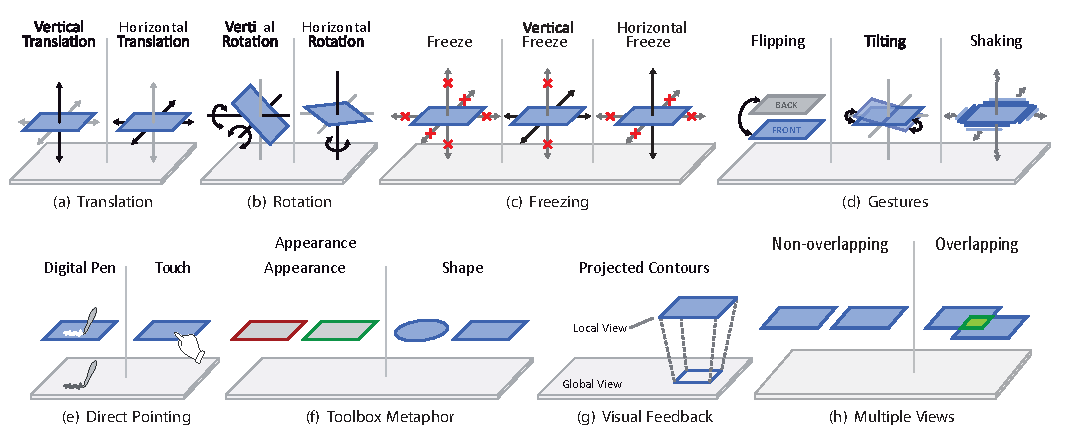
\includegraphics[width=1.0\textwidth]{figures/tangible_views_interaction.pdf}
\caption{Interaction techniques in Tangible Views (compare \protect\cite{spindler10})}
\label{fig:tangible_views_interaction}
\end{figure*}

\subsection{Steerable Tangible Interface for Multi-Layered Contents}
\cite{lee09} propose a steerable tangible interface (STI) to intuitively interact with multi-layered content projected onto a table-top display. Users can move a ring to locate to a region of interest and rotate the ring for navigating through different layers of visual information. The interaction can be compared to a magnifying glass, which is used to examine different layers of visualized content.

\begin{figure}[t]
\centering
\includegraphics[width=0.47\textwidth]{figures/sti.jpg}
\caption{An overview of the Steerable Tangible Interface (compare \protect\cite{lee09})}
\label{fig:sti}
\end{figure}

The steerable tangible interface consists of a ring with 18cm in internal radius, 1.5cm in thickness and 1cm in height. The internal circle represents a focus region, where detailed information is displayed. The ring is equipped with two LED lights to track its position and orientation. Moving the ring relocates the visualization area to the region in focus. By rotating the ring, a user can select a layer to be displayed. A Nintendo WiiRemote, installed on the ceiling,  tracks the STI. It recognizes the position of the two LEDs. With this information, the system computes the position and rotation angle of the STI. The information is displayed on a table-top display, similar to the ones described in \ref{sec:tabletop}.

\subsubsection{Application of the Steerable Tangible Interface}
The STI can be used for educational purposes. \cite{lee09} implemented a multi-layered medical education content on the system. Figure \ref{fig:sti} shows a concept of this application. Users can navigate through different layers of human body organs. If a user wants to see more detailed information beyond the skin layer, he puts the ring to the specified region. In the focus region, different views of human body information are visualized. By rotating the ring, different layers can be visualized in the region of the STI.

\subsection{G-nome Surfer}
G-nome surfer is a multi-user, multi-touch table for collaborative exploration of genomic data, presented by \cite{shaer10}. G-nome surfer allows users to compare, annotate, share, and relate genomic data. The data presented by the system includes genome visualizations, publications and gene expressions.

With G-nome surfer, scientists can collaboratively explore genomic information. Heterogeneous information can be related to each other, which simplifies comparison. Information from science databases, like abstracts of publications related to a particular gene, are also published. Through the use of touch gestures, intuitive interactions are used to simplify the exploration of complex genomic material. Figure \ref{fig:gnome} shows two students using the TUI collaboratively. G-nome surfer is implemented on the Microsoft Surface tablet platform. Several databases serve as information providers for the genomic data.

\begin{figure}[t]
\centering
\includegraphics[width=0.47\textwidth]{figures/gnome.jpg}
\caption{Students interact with G-nome surfer (compare \protect\cite{shaer10})}
\label{fig:gnome}
\end{figure}

\subsubsection{Navigation in G-nome Surfer}
G-nome surfer supports navigation of both eukaryotic and prokaryotic genomic data at multiple zoom levels. To access such data, a user selects an organism and then specifies a chromosome, range, or gene name. The view is then updated to display a portion of the chromosome with the specified gene in the center. For prokaryotes, a circular representation of the chromosome is displayed as a wheel beneath the chromosome track. With gestures, users can search through the chromosome track. Visual feedback is given all the time. By tapping on a gene, the genes sequence can be accessed. By snapping sequences together, a new windows opens with the informations aligned beneath each other.

\subsection{Augmented Chemistry - A Tangible User Interface for Chemistry Education}
Augmented Chemistry (AC) is a TUI for working and interacting with molecular models. Elements can be joined with other elements to form molecules. It was presented by \cite{fjeld02}. It consists of a set of interactive tools, which work within the system. Since many tools can be used concurrently, multiple users can work with the system at a time.

Augmented Chemistry is an augmented reality workbench consisting of a table and a rear-projection screen. Below the screen sits a camera, pointing in the users direction. The images of the camera are projected onto the screen. Therefore, the display acts as a mirror for the user. The setup can be seen in figure \ref{fig:augmented_chemistry}. The mirror image is augmented with a virtual environment. A booklet, a cube, a platform and a gripper act as the tools for interaction. Each of this tools carries one or more fiducial markers for tracking purposes. 

\subsubsection{Interaction Techniques}
Bringing two elements together triggers the composition of a molecular model. The booklet shows elements with a printed picture and a name. The user can browse the booklet with one hand. With the other hand, he can pick up an element using the gripper. When the gripper, charged with an element, is positioned near a platform holding a molecule, the element is connected with the molecule. With a rotation of the cube, users can determine where and how (single- double- or triple-binding) the element shall connect to the molecule.

Augmented Chemistry employs the ball-stick model for the visualization of molecules. In the booklet, working as an interactive menu, the valence of an atom can be seen. Atoms are visualized with a nucleus and the outmost valence shell. The representation of atoms is in accordance with the model of Bohr.